\pagebreak
\section{Code structure}
\label{app:lift_structure}
\begin{figure}[htb]
\begin{center}
\leavevmode
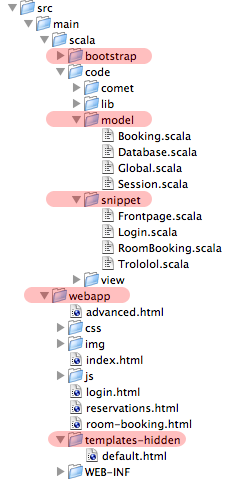
\includegraphics[width=0.4\textwidth]{images/code_structure}
\end{center}
\caption{The structure of a SBT Lift project}
\label{fig:code_structure}
\end{figure}

Figure \ref{fig:code_structure} shows the basic structure of a Lift project, using the template provided by SBT. The presentation layer is located in the webapp directory, containing the markup, graphics and design of the user interface. The templates-hidden folder contains a template file, which content is wrapped around all other pages. This is basically a header file, which should code (like menus) that should be repeated on each page.\\

The scala directory contains the server implementation. The bootstrap folder contains logic used to initialize the application, while the model and snippet folders contain the different entities of the application, and the xml bindings.